\documentclass[a4paper,11pt, notitlepage]{article}

\usepackage[utf8]{inputenc}
\usepackage[T1]{fontenc}

\usepackage[top=2.5cm, bottom=3cm, left=3cm, right=3cm, headsep=14pt]{geometry}
\usepackage{graphicx}
\graphicspath{{images/}}
\usepackage[export]{adjustbox}

\usepackage{datetime}
\usepackage{float}
\usepackage{a4wide}
\usepackage[super]{nth}
\usepackage{mathtools}
\usepackage{hyperref}
\usepackage{fancyvrb}
\usepackage{booktabs}
\usepackage{multirow}
\usepackage{caption}

\usepackage{natbib}
\bibliographystyle{unsrt}


\setlength{\parskip}{0.5em}

\begin{document}

\title{
\vspace{-3cm}
Report 1 - OpenMP}
\author{Nguyen Nhu Khoa - M.ICT.06.003}
\maketitle

\pagestyle{plain}
\setcounter{page}{1}

\vspace{-1cm}
\newdate{date}{31}{10}{2017}
\noindent

\section{OpenMP Implementation}

\begin{verbatim}
void Labwork::labwork1_OpenMP() {
    int pixelCount = inputImage->width * inputImage->height;
    outputImage = static_cast<char *>(malloc(pixelCount * 3));
    for (int j = 0; j < 100; j++) {   
        #pragma omp parallel for
        for (int i = 0; i < pixelCount; i++) {
            outputImage[i * 3] = (char) (((int) inputImage->buffer[i * 3] + 
            							(int) inputImage->buffer[i * 3 + 1] +
                                     (int) inputImage->buffer[i * 3 + 2]) / 3);
            outputImage[i * 3 + 1] = outputImage[i * 3];
            outputImage[i * 3 + 2] = outputImage[i * 3];
        }
    }
}
\end{verbatim}

\section{Speed Up result}
\begin{verbatim}
labwork 1 CPU ellapsed 5758.0ms
labwork 1 CPU-OMP ellapsed 2124.7ms
\end{verbatim}
~\\
So, the speed up for adding a simple static OMP directive is approximately 2.7x.

\section{Testing other configuration}

\begin{figure}[H]
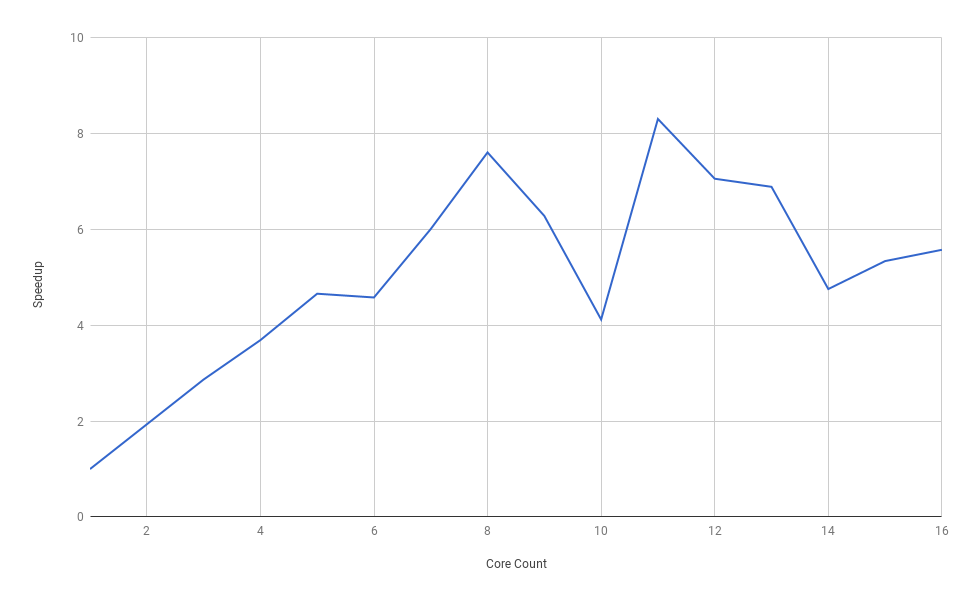
\includegraphics[width=15cm]{chart.png}
\centering
\caption{Speedup with different core counts and scheduling}
\end{figure}

\end{document}